% Graphic for TeX using PGF
% Title: C:\Users\nicolas\Desktop\RayTracing\diagrams\Diagramme1.dia
% Creator: Dia v0.97.2
% CreationDate: Sat Feb 06 20:37:32 2016
% For: nicolas
% \usepackage{tikz}
% The following commands are not supported in PSTricks at present
% We define them conditionally, so when they are implemented,
% this pgf file will use them.
\ifx\du\undefined
  \newlength{\du}
\fi
\setlength{\du}{15\unitlength}
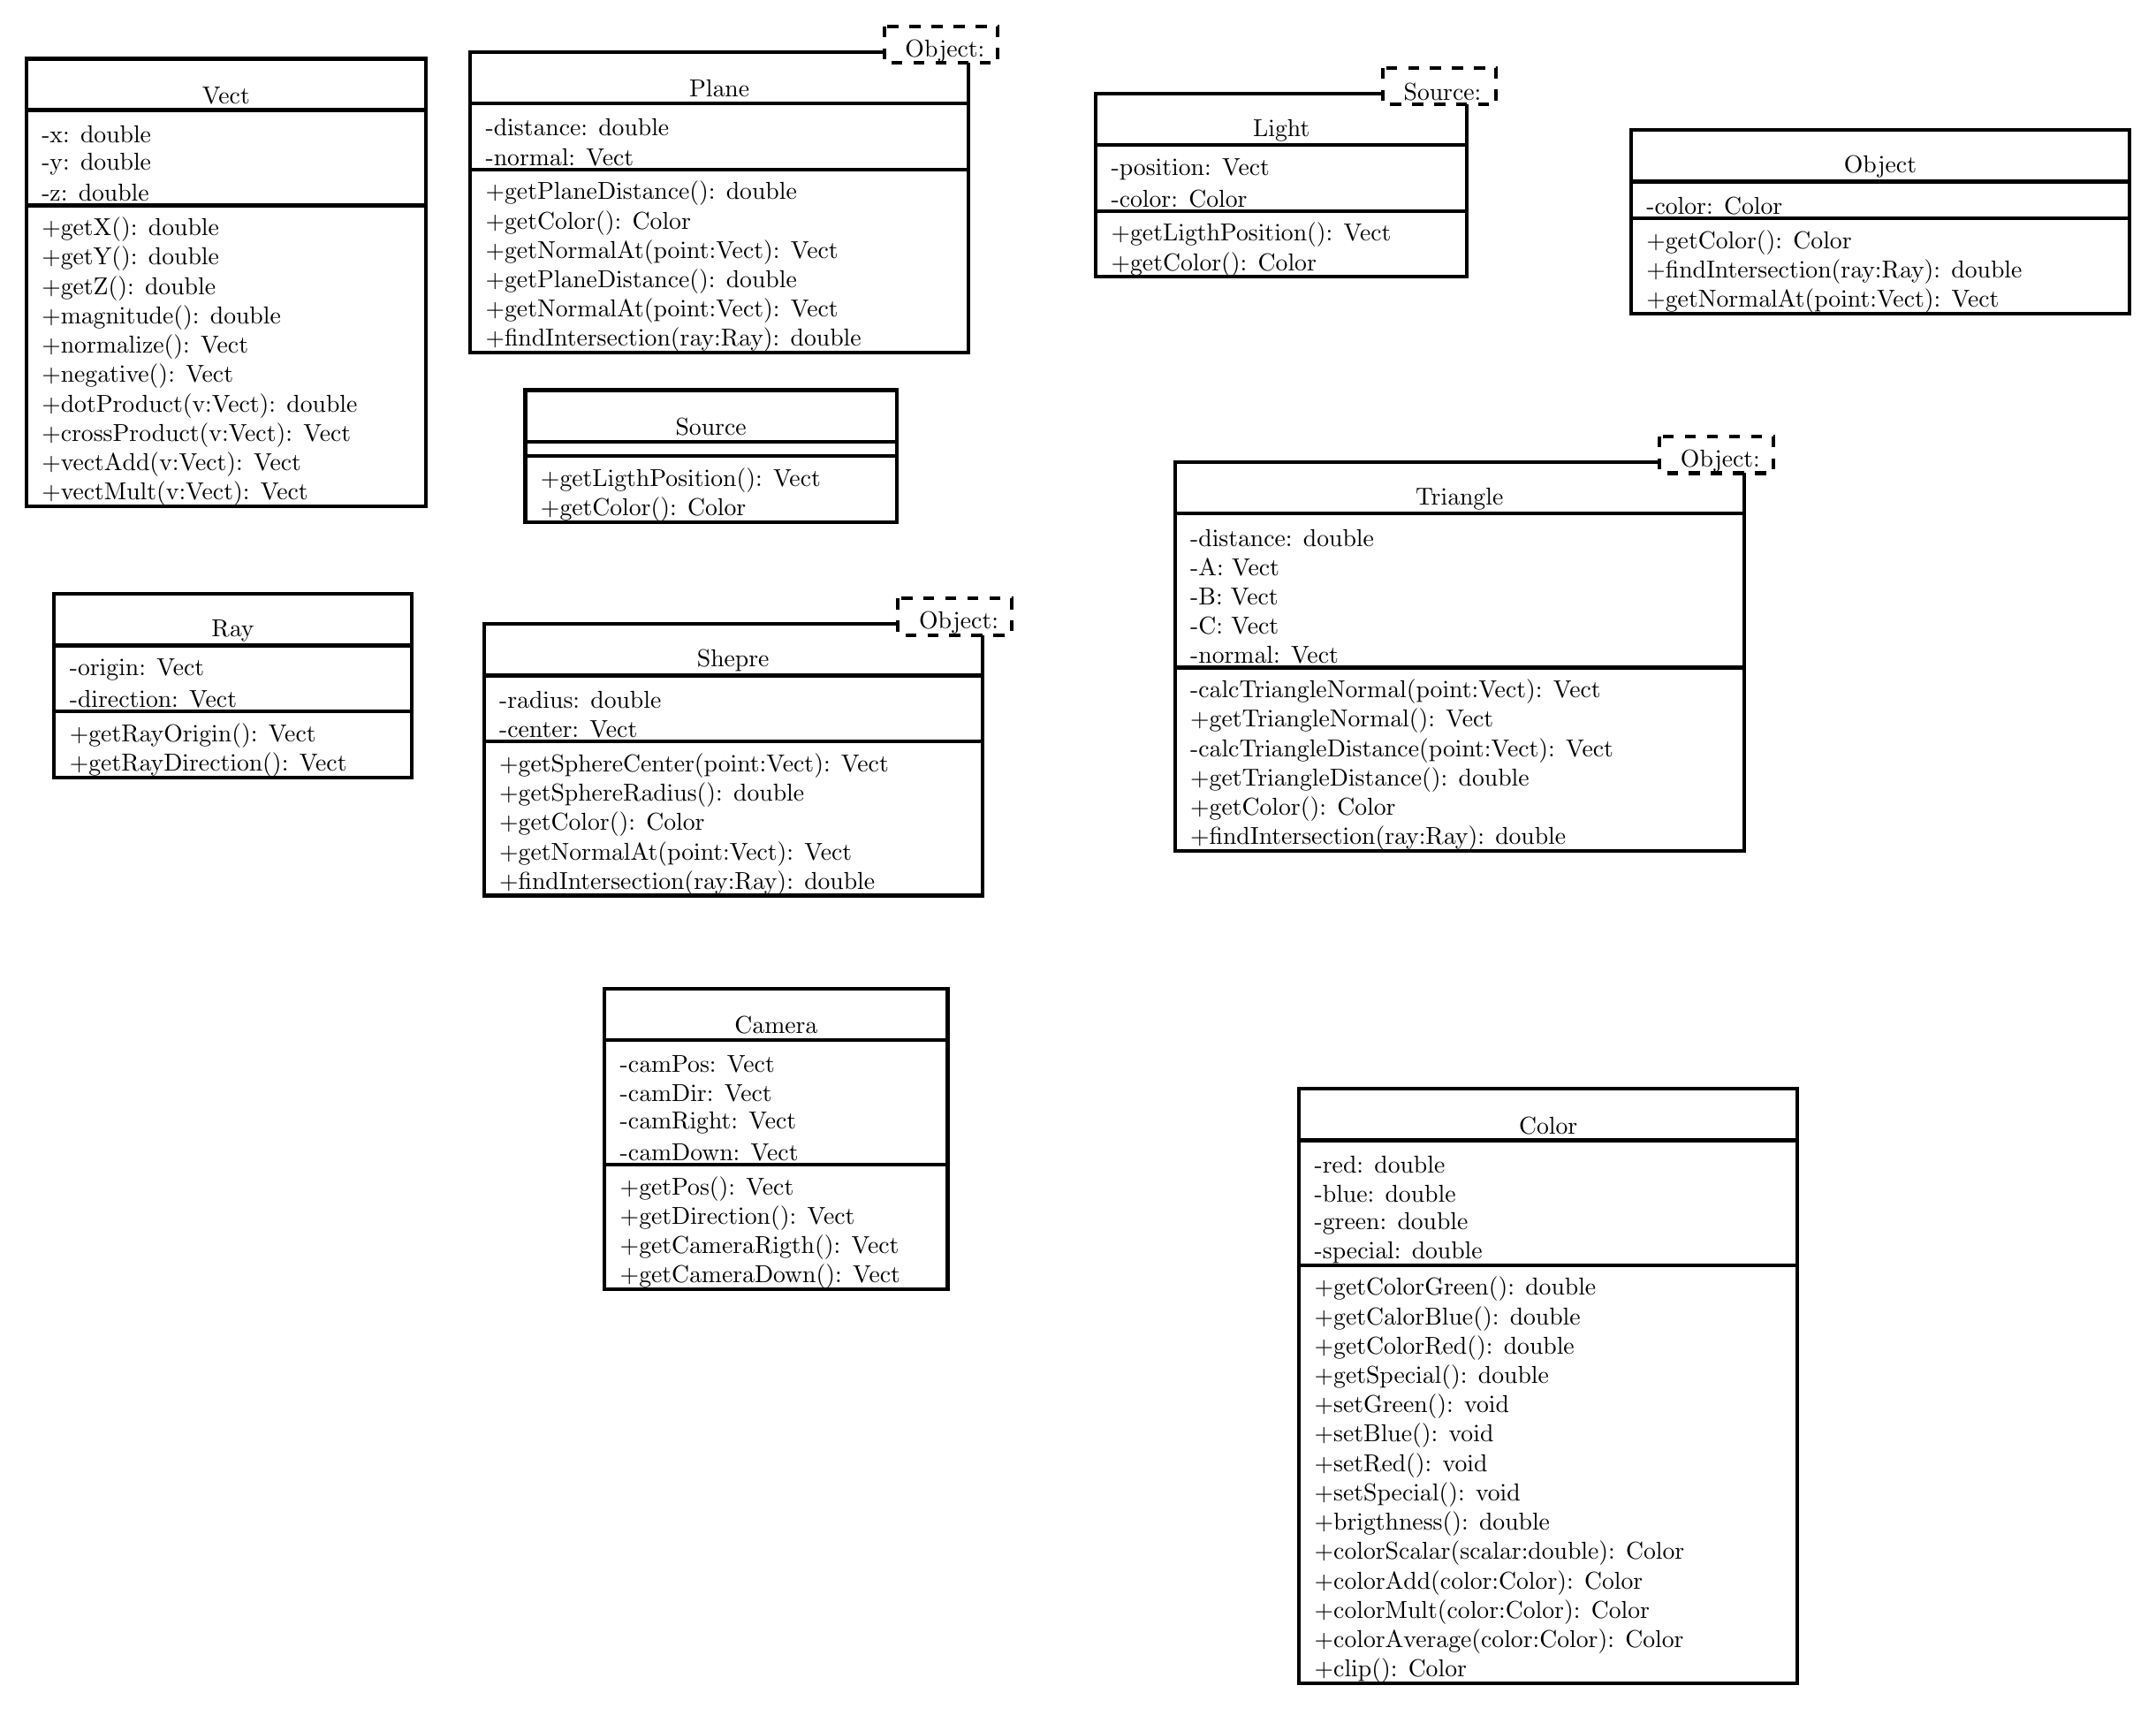
\begin{tikzpicture}
\pgftransformxscale{1.000000}
\pgftransformyscale{-1.000000}
\definecolor{dialinecolor}{rgb}{0.000000, 0.000000, 0.000000}
\pgfsetstrokecolor{dialinecolor}
\definecolor{dialinecolor}{rgb}{1.000000, 1.000000, 1.000000}
\pgfsetfillcolor{dialinecolor}
\pgfsetlinewidth{0.100000\du}
\pgfsetdash{}{0pt}
\definecolor{dialinecolor}{rgb}{1.000000, 1.000000, 1.000000}
\pgfsetfillcolor{dialinecolor}
\fill (47.516500\du,4.057720\du)--(47.516500\du,5.457720\du)--(61.106500\du,5.457720\du)--(61.106500\du,4.057720\du)--cycle;
\definecolor{dialinecolor}{rgb}{0.000000, 0.000000, 0.000000}
\pgfsetstrokecolor{dialinecolor}
\draw (47.516500\du,4.057720\du)--(47.516500\du,5.457720\du)--(61.106500\du,5.457720\du)--(61.106500\du,4.057720\du)--cycle;
% setfont left to latex
\definecolor{dialinecolor}{rgb}{0.000000, 0.000000, 0.000000}
\pgfsetstrokecolor{dialinecolor}
\node at (54.311500\du,5.057720\du){Object};
\definecolor{dialinecolor}{rgb}{1.000000, 1.000000, 1.000000}
\pgfsetfillcolor{dialinecolor}
\fill (47.516500\du,5.457720\du)--(47.516500\du,6.457720\du)--(61.106500\du,6.457720\du)--(61.106500\du,5.457720\du)--cycle;
\definecolor{dialinecolor}{rgb}{0.000000, 0.000000, 0.000000}
\pgfsetstrokecolor{dialinecolor}
\draw (47.516500\du,5.457720\du)--(47.516500\du,6.457720\du)--(61.106500\du,6.457720\du)--(61.106500\du,5.457720\du)--cycle;
% setfont left to latex
\definecolor{dialinecolor}{rgb}{0.000000, 0.000000, 0.000000}
\pgfsetstrokecolor{dialinecolor}
\node[anchor=west] at (47.666500\du,6.117720\du){-color: Color};
\definecolor{dialinecolor}{rgb}{1.000000, 1.000000, 1.000000}
\pgfsetfillcolor{dialinecolor}
\fill (47.516500\du,6.457720\du)--(47.516500\du,9.057720\du)--(61.106500\du,9.057720\du)--(61.106500\du,6.457720\du)--cycle;
\definecolor{dialinecolor}{rgb}{0.000000, 0.000000, 0.000000}
\pgfsetstrokecolor{dialinecolor}
\draw (47.516500\du,6.457720\du)--(47.516500\du,9.057720\du)--(61.106500\du,9.057720\du)--(61.106500\du,6.457720\du)--cycle;
% setfont left to latex
\definecolor{dialinecolor}{rgb}{0.000000, 0.000000, 0.000000}
\pgfsetstrokecolor{dialinecolor}
\node[anchor=west] at (47.666500\du,7.117720\du){+getColor(): Color};
% setfont left to latex
\definecolor{dialinecolor}{rgb}{0.000000, 0.000000, 0.000000}
\pgfsetstrokecolor{dialinecolor}
\node[anchor=west] at (47.666500\du,7.917720\du){+findIntersection(ray:Ray): double};
% setfont left to latex
\definecolor{dialinecolor}{rgb}{0.000000, 0.000000, 0.000000}
\pgfsetstrokecolor{dialinecolor}
\node[anchor=west] at (47.666500\du,8.717720\du){+getNormalAt(point:Vect): Vect};
\pgfsetlinewidth{0.100000\du}
\pgfsetdash{}{0pt}
\definecolor{dialinecolor}{rgb}{1.000000, 1.000000, 1.000000}
\pgfsetfillcolor{dialinecolor}
\fill (15.868000\du,1.925010\du)--(15.868000\du,3.325010\du)--(29.458000\du,3.325010\du)--(29.458000\du,1.925010\du)--cycle;
\definecolor{dialinecolor}{rgb}{0.000000, 0.000000, 0.000000}
\pgfsetstrokecolor{dialinecolor}
\draw (15.868000\du,1.925010\du)--(15.868000\du,3.325010\du)--(29.458000\du,3.325010\du)--(29.458000\du,1.925010\du)--cycle;
% setfont left to latex
\definecolor{dialinecolor}{rgb}{0.000000, 0.000000, 0.000000}
\pgfsetstrokecolor{dialinecolor}
\node at (22.663000\du,2.925010\du){Plane};
\definecolor{dialinecolor}{rgb}{1.000000, 1.000000, 1.000000}
\pgfsetfillcolor{dialinecolor}
\fill (15.868000\du,3.325010\du)--(15.868000\du,5.125010\du)--(29.458000\du,5.125010\du)--(29.458000\du,3.325010\du)--cycle;
\definecolor{dialinecolor}{rgb}{0.000000, 0.000000, 0.000000}
\pgfsetstrokecolor{dialinecolor}
\draw (15.868000\du,3.325010\du)--(15.868000\du,5.125010\du)--(29.458000\du,5.125010\du)--(29.458000\du,3.325010\du)--cycle;
% setfont left to latex
\definecolor{dialinecolor}{rgb}{0.000000, 0.000000, 0.000000}
\pgfsetstrokecolor{dialinecolor}
\node[anchor=west] at (16.018000\du,3.985010\du){-distance: double};
% setfont left to latex
\definecolor{dialinecolor}{rgb}{0.000000, 0.000000, 0.000000}
\pgfsetstrokecolor{dialinecolor}
\node[anchor=west] at (16.018000\du,4.785010\du){-normal: Vect};
\definecolor{dialinecolor}{rgb}{1.000000, 1.000000, 1.000000}
\pgfsetfillcolor{dialinecolor}
\fill (15.868000\du,5.125010\du)--(15.868000\du,10.125010\du)--(29.458000\du,10.125010\du)--(29.458000\du,5.125010\du)--cycle;
\definecolor{dialinecolor}{rgb}{0.000000, 0.000000, 0.000000}
\pgfsetstrokecolor{dialinecolor}
\draw (15.868000\du,5.125010\du)--(15.868000\du,10.125010\du)--(29.458000\du,10.125010\du)--(29.458000\du,5.125010\du)--cycle;
% setfont left to latex
\definecolor{dialinecolor}{rgb}{0.000000, 0.000000, 0.000000}
\pgfsetstrokecolor{dialinecolor}
\node[anchor=west] at (16.018000\du,5.785010\du){+getPlaneDistance(): double};
% setfont left to latex
\definecolor{dialinecolor}{rgb}{0.000000, 0.000000, 0.000000}
\pgfsetstrokecolor{dialinecolor}
\node[anchor=west] at (16.018000\du,6.585010\du){+getColor(): Color};
% setfont left to latex
\definecolor{dialinecolor}{rgb}{0.000000, 0.000000, 0.000000}
\pgfsetstrokecolor{dialinecolor}
\node[anchor=west] at (16.018000\du,7.385010\du){+getNormalAt(point:Vect): Vect};
% setfont left to latex
\definecolor{dialinecolor}{rgb}{0.000000, 0.000000, 0.000000}
\pgfsetstrokecolor{dialinecolor}
\node[anchor=west] at (16.018000\du,8.185010\du){+getPlaneDistance(): double};
% setfont left to latex
\definecolor{dialinecolor}{rgb}{0.000000, 0.000000, 0.000000}
\pgfsetstrokecolor{dialinecolor}
\node[anchor=west] at (16.018000\du,8.985010\du){+getNormalAt(point:Vect): Vect};
% setfont left to latex
\definecolor{dialinecolor}{rgb}{0.000000, 0.000000, 0.000000}
\pgfsetstrokecolor{dialinecolor}
\node[anchor=west] at (16.018000\du,9.785010\du){+findIntersection(ray:Ray): double};
\definecolor{dialinecolor}{rgb}{1.000000, 1.000000, 1.000000}
\pgfsetfillcolor{dialinecolor}
\fill (27.158000\du,1.225010\du)--(27.158000\du,2.225010\du)--(30.253000\du,2.225010\du)--(30.253000\du,1.225010\du)--cycle;
\pgfsetdash{{1.000000\du}{1.000000\du}}{0\du}
\pgfsetdash{{0.300000\du}{0.300000\du}}{0\du}
\definecolor{dialinecolor}{rgb}{0.000000, 0.000000, 0.000000}
\pgfsetstrokecolor{dialinecolor}
\draw (27.158000\du,1.225010\du)--(27.158000\du,2.225010\du)--(30.253000\du,2.225010\du)--(30.253000\du,1.225010\du)--cycle;
% setfont left to latex
\definecolor{dialinecolor}{rgb}{0.000000, 0.000000, 0.000000}
\pgfsetstrokecolor{dialinecolor}
\node[anchor=west] at (27.458000\du,1.885010\du){Object:};
\pgfsetlinewidth{0.100000\du}
\pgfsetdash{}{0pt}
\definecolor{dialinecolor}{rgb}{1.000000, 1.000000, 1.000000}
\pgfsetfillcolor{dialinecolor}
\fill (16.243400\du,17.523800\du)--(16.243400\du,18.923800\du)--(29.833400\du,18.923800\du)--(29.833400\du,17.523800\du)--cycle;
\definecolor{dialinecolor}{rgb}{0.000000, 0.000000, 0.000000}
\pgfsetstrokecolor{dialinecolor}
\draw (16.243400\du,17.523800\du)--(16.243400\du,18.923800\du)--(29.833400\du,18.923800\du)--(29.833400\du,17.523800\du)--cycle;
% setfont left to latex
\definecolor{dialinecolor}{rgb}{0.000000, 0.000000, 0.000000}
\pgfsetstrokecolor{dialinecolor}
\node at (23.038400\du,18.523800\du){Shepre};
\definecolor{dialinecolor}{rgb}{1.000000, 1.000000, 1.000000}
\pgfsetfillcolor{dialinecolor}
\fill (16.243400\du,18.923800\du)--(16.243400\du,20.723800\du)--(29.833400\du,20.723800\du)--(29.833400\du,18.923800\du)--cycle;
\definecolor{dialinecolor}{rgb}{0.000000, 0.000000, 0.000000}
\pgfsetstrokecolor{dialinecolor}
\draw (16.243400\du,18.923800\du)--(16.243400\du,20.723800\du)--(29.833400\du,20.723800\du)--(29.833400\du,18.923800\du)--cycle;
% setfont left to latex
\definecolor{dialinecolor}{rgb}{0.000000, 0.000000, 0.000000}
\pgfsetstrokecolor{dialinecolor}
\node[anchor=west] at (16.393400\du,19.583800\du){-radius: double};
% setfont left to latex
\definecolor{dialinecolor}{rgb}{0.000000, 0.000000, 0.000000}
\pgfsetstrokecolor{dialinecolor}
\node[anchor=west] at (16.393400\du,20.383800\du){-center: Vect};
\definecolor{dialinecolor}{rgb}{1.000000, 1.000000, 1.000000}
\pgfsetfillcolor{dialinecolor}
\fill (16.243400\du,20.723800\du)--(16.243400\du,24.923800\du)--(29.833400\du,24.923800\du)--(29.833400\du,20.723800\du)--cycle;
\definecolor{dialinecolor}{rgb}{0.000000, 0.000000, 0.000000}
\pgfsetstrokecolor{dialinecolor}
\draw (16.243400\du,20.723800\du)--(16.243400\du,24.923800\du)--(29.833400\du,24.923800\du)--(29.833400\du,20.723800\du)--cycle;
% setfont left to latex
\definecolor{dialinecolor}{rgb}{0.000000, 0.000000, 0.000000}
\pgfsetstrokecolor{dialinecolor}
\node[anchor=west] at (16.393400\du,21.383800\du){+getSphereCenter(point:Vect): Vect};
% setfont left to latex
\definecolor{dialinecolor}{rgb}{0.000000, 0.000000, 0.000000}
\pgfsetstrokecolor{dialinecolor}
\node[anchor=west] at (16.393400\du,22.183800\du){+getSphereRadius(): double};
% setfont left to latex
\definecolor{dialinecolor}{rgb}{0.000000, 0.000000, 0.000000}
\pgfsetstrokecolor{dialinecolor}
\node[anchor=west] at (16.393400\du,22.983800\du){+getColor(): Color};
% setfont left to latex
\definecolor{dialinecolor}{rgb}{0.000000, 0.000000, 0.000000}
\pgfsetstrokecolor{dialinecolor}
\node[anchor=west] at (16.393400\du,23.783800\du){+getNormalAt(point:Vect): Vect};
% setfont left to latex
\definecolor{dialinecolor}{rgb}{0.000000, 0.000000, 0.000000}
\pgfsetstrokecolor{dialinecolor}
\node[anchor=west] at (16.393400\du,24.583800\du){+findIntersection(ray:Ray): double};
\definecolor{dialinecolor}{rgb}{1.000000, 1.000000, 1.000000}
\pgfsetfillcolor{dialinecolor}
\fill (27.533400\du,16.823800\du)--(27.533400\du,17.823800\du)--(30.628400\du,17.823800\du)--(30.628400\du,16.823800\du)--cycle;
\pgfsetdash{{0.300000\du}{0.300000\du}}{0\du}
\pgfsetdash{{0.300000\du}{0.300000\du}}{0\du}
\definecolor{dialinecolor}{rgb}{0.000000, 0.000000, 0.000000}
\pgfsetstrokecolor{dialinecolor}
\draw (27.533400\du,16.823800\du)--(27.533400\du,17.823800\du)--(30.628400\du,17.823800\du)--(30.628400\du,16.823800\du)--cycle;
% setfont left to latex
\definecolor{dialinecolor}{rgb}{0.000000, 0.000000, 0.000000}
\pgfsetstrokecolor{dialinecolor}
\node[anchor=west] at (27.833400\du,17.483800\du){Object:};
\pgfsetlinewidth{0.100000\du}
\pgfsetdash{}{0pt}
\definecolor{dialinecolor}{rgb}{1.000000, 1.000000, 1.000000}
\pgfsetfillcolor{dialinecolor}
\fill (35.082000\du,13.107200\du)--(35.082000\du,14.507200\du)--(50.597000\du,14.507200\du)--(50.597000\du,13.107200\du)--cycle;
\definecolor{dialinecolor}{rgb}{0.000000, 0.000000, 0.000000}
\pgfsetstrokecolor{dialinecolor}
\draw (35.082000\du,13.107200\du)--(35.082000\du,14.507200\du)--(50.597000\du,14.507200\du)--(50.597000\du,13.107200\du)--cycle;
% setfont left to latex
\definecolor{dialinecolor}{rgb}{0.000000, 0.000000, 0.000000}
\pgfsetstrokecolor{dialinecolor}
\node at (42.839500\du,14.107200\du){Triangle};
\definecolor{dialinecolor}{rgb}{1.000000, 1.000000, 1.000000}
\pgfsetfillcolor{dialinecolor}
\fill (35.082000\du,14.507200\du)--(35.082000\du,18.707200\du)--(50.597000\du,18.707200\du)--(50.597000\du,14.507200\du)--cycle;
\definecolor{dialinecolor}{rgb}{0.000000, 0.000000, 0.000000}
\pgfsetstrokecolor{dialinecolor}
\draw (35.082000\du,14.507200\du)--(35.082000\du,18.707200\du)--(50.597000\du,18.707200\du)--(50.597000\du,14.507200\du)--cycle;
% setfont left to latex
\definecolor{dialinecolor}{rgb}{0.000000, 0.000000, 0.000000}
\pgfsetstrokecolor{dialinecolor}
\node[anchor=west] at (35.232000\du,15.167200\du){-distance: double};
% setfont left to latex
\definecolor{dialinecolor}{rgb}{0.000000, 0.000000, 0.000000}
\pgfsetstrokecolor{dialinecolor}
\node[anchor=west] at (35.232000\du,15.967200\du){-A: Vect};
% setfont left to latex
\definecolor{dialinecolor}{rgb}{0.000000, 0.000000, 0.000000}
\pgfsetstrokecolor{dialinecolor}
\node[anchor=west] at (35.232000\du,16.767200\du){-B: Vect};
% setfont left to latex
\definecolor{dialinecolor}{rgb}{0.000000, 0.000000, 0.000000}
\pgfsetstrokecolor{dialinecolor}
\node[anchor=west] at (35.232000\du,17.567200\du){-C: Vect};
% setfont left to latex
\definecolor{dialinecolor}{rgb}{0.000000, 0.000000, 0.000000}
\pgfsetstrokecolor{dialinecolor}
\node[anchor=west] at (35.232000\du,18.367200\du){-normal: Vect};
\definecolor{dialinecolor}{rgb}{1.000000, 1.000000, 1.000000}
\pgfsetfillcolor{dialinecolor}
\fill (35.082000\du,18.707200\du)--(35.082000\du,23.707200\du)--(50.597000\du,23.707200\du)--(50.597000\du,18.707200\du)--cycle;
\definecolor{dialinecolor}{rgb}{0.000000, 0.000000, 0.000000}
\pgfsetstrokecolor{dialinecolor}
\draw (35.082000\du,18.707200\du)--(35.082000\du,23.707200\du)--(50.597000\du,23.707200\du)--(50.597000\du,18.707200\du)--cycle;
% setfont left to latex
\definecolor{dialinecolor}{rgb}{0.000000, 0.000000, 0.000000}
\pgfsetstrokecolor{dialinecolor}
\node[anchor=west] at (35.232000\du,19.367200\du){-calcTriangleNormal(point:Vect): Vect};
% setfont left to latex
\definecolor{dialinecolor}{rgb}{0.000000, 0.000000, 0.000000}
\pgfsetstrokecolor{dialinecolor}
\node[anchor=west] at (35.232000\du,20.167200\du){+getTriangleNormal(): Vect};
% setfont left to latex
\definecolor{dialinecolor}{rgb}{0.000000, 0.000000, 0.000000}
\pgfsetstrokecolor{dialinecolor}
\node[anchor=west] at (35.232000\du,20.967200\du){-calcTriangleDistance(point:Vect): Vect};
% setfont left to latex
\definecolor{dialinecolor}{rgb}{0.000000, 0.000000, 0.000000}
\pgfsetstrokecolor{dialinecolor}
\node[anchor=west] at (35.232000\du,21.767200\du){+getTriangleDistance(): double};
% setfont left to latex
\definecolor{dialinecolor}{rgb}{0.000000, 0.000000, 0.000000}
\pgfsetstrokecolor{dialinecolor}
\node[anchor=west] at (35.232000\du,22.567200\du){+getColor(): Color};
% setfont left to latex
\definecolor{dialinecolor}{rgb}{0.000000, 0.000000, 0.000000}
\pgfsetstrokecolor{dialinecolor}
\node[anchor=west] at (35.232000\du,23.367200\du){+findIntersection(ray:Ray): double};
\definecolor{dialinecolor}{rgb}{1.000000, 1.000000, 1.000000}
\pgfsetfillcolor{dialinecolor}
\fill (48.297000\du,12.407200\du)--(48.297000\du,13.407200\du)--(51.392000\du,13.407200\du)--(51.392000\du,12.407200\du)--cycle;
\pgfsetdash{{0.300000\du}{0.300000\du}}{0\du}
\pgfsetdash{{0.300000\du}{0.300000\du}}{0\du}
\definecolor{dialinecolor}{rgb}{0.000000, 0.000000, 0.000000}
\pgfsetstrokecolor{dialinecolor}
\draw (48.297000\du,12.407200\du)--(48.297000\du,13.407200\du)--(51.392000\du,13.407200\du)--(51.392000\du,12.407200\du)--cycle;
% setfont left to latex
\definecolor{dialinecolor}{rgb}{0.000000, 0.000000, 0.000000}
\pgfsetstrokecolor{dialinecolor}
\node[anchor=west] at (48.597000\du,13.067200\du){Object:};
\pgfsetlinewidth{0.100000\du}
\pgfsetdash{}{0pt}
\definecolor{dialinecolor}{rgb}{1.000000, 1.000000, 1.000000}
\pgfsetfillcolor{dialinecolor}
\fill (3.767170\du,2.108660\du)--(3.767170\du,3.508660\du)--(14.662170\du,3.508660\du)--(14.662170\du,2.108660\du)--cycle;
\definecolor{dialinecolor}{rgb}{0.000000, 0.000000, 0.000000}
\pgfsetstrokecolor{dialinecolor}
\draw (3.767170\du,2.108660\du)--(3.767170\du,3.508660\du)--(14.662170\du,3.508660\du)--(14.662170\du,2.108660\du)--cycle;
% setfont left to latex
\definecolor{dialinecolor}{rgb}{0.000000, 0.000000, 0.000000}
\pgfsetstrokecolor{dialinecolor}
\node at (9.214670\du,3.108660\du){Vect};
\definecolor{dialinecolor}{rgb}{1.000000, 1.000000, 1.000000}
\pgfsetfillcolor{dialinecolor}
\fill (3.767170\du,3.508660\du)--(3.767170\du,6.108660\du)--(14.662170\du,6.108660\du)--(14.662170\du,3.508660\du)--cycle;
\definecolor{dialinecolor}{rgb}{0.000000, 0.000000, 0.000000}
\pgfsetstrokecolor{dialinecolor}
\draw (3.767170\du,3.508660\du)--(3.767170\du,6.108660\du)--(14.662170\du,6.108660\du)--(14.662170\du,3.508660\du)--cycle;
% setfont left to latex
\definecolor{dialinecolor}{rgb}{0.000000, 0.000000, 0.000000}
\pgfsetstrokecolor{dialinecolor}
\node[anchor=west] at (3.917170\du,4.168660\du){-x: double};
% setfont left to latex
\definecolor{dialinecolor}{rgb}{0.000000, 0.000000, 0.000000}
\pgfsetstrokecolor{dialinecolor}
\node[anchor=west] at (3.917170\du,4.968660\du){-y: double};
% setfont left to latex
\definecolor{dialinecolor}{rgb}{0.000000, 0.000000, 0.000000}
\pgfsetstrokecolor{dialinecolor}
\node[anchor=west] at (3.917170\du,5.768660\du){-z: double};
\definecolor{dialinecolor}{rgb}{1.000000, 1.000000, 1.000000}
\pgfsetfillcolor{dialinecolor}
\fill (3.767170\du,6.108660\du)--(3.767170\du,14.308660\du)--(14.662170\du,14.308660\du)--(14.662170\du,6.108660\du)--cycle;
\definecolor{dialinecolor}{rgb}{0.000000, 0.000000, 0.000000}
\pgfsetstrokecolor{dialinecolor}
\draw (3.767170\du,6.108660\du)--(3.767170\du,14.308660\du)--(14.662170\du,14.308660\du)--(14.662170\du,6.108660\du)--cycle;
% setfont left to latex
\definecolor{dialinecolor}{rgb}{0.000000, 0.000000, 0.000000}
\pgfsetstrokecolor{dialinecolor}
\node[anchor=west] at (3.917170\du,6.768660\du){+getX(): double};
% setfont left to latex
\definecolor{dialinecolor}{rgb}{0.000000, 0.000000, 0.000000}
\pgfsetstrokecolor{dialinecolor}
\node[anchor=west] at (3.917170\du,7.568660\du){+getY(): double};
% setfont left to latex
\definecolor{dialinecolor}{rgb}{0.000000, 0.000000, 0.000000}
\pgfsetstrokecolor{dialinecolor}
\node[anchor=west] at (3.917170\du,8.368660\du){+getZ(): double};
% setfont left to latex
\definecolor{dialinecolor}{rgb}{0.000000, 0.000000, 0.000000}
\pgfsetstrokecolor{dialinecolor}
\node[anchor=west] at (3.917170\du,9.168660\du){+magnitude(): double};
% setfont left to latex
\definecolor{dialinecolor}{rgb}{0.000000, 0.000000, 0.000000}
\pgfsetstrokecolor{dialinecolor}
\node[anchor=west] at (3.917170\du,9.968660\du){+normalize(): Vect};
% setfont left to latex
\definecolor{dialinecolor}{rgb}{0.000000, 0.000000, 0.000000}
\pgfsetstrokecolor{dialinecolor}
\node[anchor=west] at (3.917170\du,10.768660\du){+negative(): Vect};
% setfont left to latex
\definecolor{dialinecolor}{rgb}{0.000000, 0.000000, 0.000000}
\pgfsetstrokecolor{dialinecolor}
\node[anchor=west] at (3.917170\du,11.568660\du){+dotProduct(v:Vect): double};
% setfont left to latex
\definecolor{dialinecolor}{rgb}{0.000000, 0.000000, 0.000000}
\pgfsetstrokecolor{dialinecolor}
\node[anchor=west] at (3.917170\du,12.368660\du){+crossProduct(v:Vect): Vect};
% setfont left to latex
\definecolor{dialinecolor}{rgb}{0.000000, 0.000000, 0.000000}
\pgfsetstrokecolor{dialinecolor}
\node[anchor=west] at (3.917170\du,13.168660\du){+vectAdd(v:Vect): Vect};
% setfont left to latex
\definecolor{dialinecolor}{rgb}{0.000000, 0.000000, 0.000000}
\pgfsetstrokecolor{dialinecolor}
\node[anchor=west] at (3.917170\du,13.968660\du){+vectMult(v:Vect): Vect};
\pgfsetlinewidth{0.100000\du}
\pgfsetdash{}{0pt}
\definecolor{dialinecolor}{rgb}{1.000000, 1.000000, 1.000000}
\pgfsetfillcolor{dialinecolor}
\fill (4.527710\du,16.706000\du)--(4.527710\du,18.106000\du)--(14.267710\du,18.106000\du)--(14.267710\du,16.706000\du)--cycle;
\definecolor{dialinecolor}{rgb}{0.000000, 0.000000, 0.000000}
\pgfsetstrokecolor{dialinecolor}
\draw (4.527710\du,16.706000\du)--(4.527710\du,18.106000\du)--(14.267710\du,18.106000\du)--(14.267710\du,16.706000\du)--cycle;
% setfont left to latex
\definecolor{dialinecolor}{rgb}{0.000000, 0.000000, 0.000000}
\pgfsetstrokecolor{dialinecolor}
\node at (9.397710\du,17.706000\du){Ray};
\definecolor{dialinecolor}{rgb}{1.000000, 1.000000, 1.000000}
\pgfsetfillcolor{dialinecolor}
\fill (4.527710\du,18.106000\du)--(4.527710\du,19.906000\du)--(14.267710\du,19.906000\du)--(14.267710\du,18.106000\du)--cycle;
\definecolor{dialinecolor}{rgb}{0.000000, 0.000000, 0.000000}
\pgfsetstrokecolor{dialinecolor}
\draw (4.527710\du,18.106000\du)--(4.527710\du,19.906000\du)--(14.267710\du,19.906000\du)--(14.267710\du,18.106000\du)--cycle;
% setfont left to latex
\definecolor{dialinecolor}{rgb}{0.000000, 0.000000, 0.000000}
\pgfsetstrokecolor{dialinecolor}
\node[anchor=west] at (4.677710\du,18.766000\du){-origin: Vect};
% setfont left to latex
\definecolor{dialinecolor}{rgb}{0.000000, 0.000000, 0.000000}
\pgfsetstrokecolor{dialinecolor}
\node[anchor=west] at (4.677710\du,19.566000\du){-direction: Vect};
\definecolor{dialinecolor}{rgb}{1.000000, 1.000000, 1.000000}
\pgfsetfillcolor{dialinecolor}
\fill (4.527710\du,19.906000\du)--(4.527710\du,21.706000\du)--(14.267710\du,21.706000\du)--(14.267710\du,19.906000\du)--cycle;
\definecolor{dialinecolor}{rgb}{0.000000, 0.000000, 0.000000}
\pgfsetstrokecolor{dialinecolor}
\draw (4.527710\du,19.906000\du)--(4.527710\du,21.706000\du)--(14.267710\du,21.706000\du)--(14.267710\du,19.906000\du)--cycle;
% setfont left to latex
\definecolor{dialinecolor}{rgb}{0.000000, 0.000000, 0.000000}
\pgfsetstrokecolor{dialinecolor}
\node[anchor=west] at (4.677710\du,20.566000\du){+getRayOrigin(): Vect};
% setfont left to latex
\definecolor{dialinecolor}{rgb}{0.000000, 0.000000, 0.000000}
\pgfsetstrokecolor{dialinecolor}
\node[anchor=west] at (4.677710\du,21.366000\du){+getRayDirection(): Vect};
\pgfsetlinewidth{0.100000\du}
\pgfsetdash{}{0pt}
\definecolor{dialinecolor}{rgb}{1.000000, 1.000000, 1.000000}
\pgfsetfillcolor{dialinecolor}
\fill (17.370900\du,11.145700\du)--(17.370900\du,12.545700\du)--(27.495900\du,12.545700\du)--(27.495900\du,11.145700\du)--cycle;
\definecolor{dialinecolor}{rgb}{0.000000, 0.000000, 0.000000}
\pgfsetstrokecolor{dialinecolor}
\draw (17.370900\du,11.145700\du)--(17.370900\du,12.545700\du)--(27.495900\du,12.545700\du)--(27.495900\du,11.145700\du)--cycle;
% setfont left to latex
\definecolor{dialinecolor}{rgb}{0.000000, 0.000000, 0.000000}
\pgfsetstrokecolor{dialinecolor}
\node at (22.433400\du,12.145700\du){Source};
\definecolor{dialinecolor}{rgb}{1.000000, 1.000000, 1.000000}
\pgfsetfillcolor{dialinecolor}
\fill (17.370900\du,12.545700\du)--(17.370900\du,12.945700\du)--(27.495900\du,12.945700\du)--(27.495900\du,12.545700\du)--cycle;
\definecolor{dialinecolor}{rgb}{0.000000, 0.000000, 0.000000}
\pgfsetstrokecolor{dialinecolor}
\draw (17.370900\du,12.545700\du)--(17.370900\du,12.945700\du)--(27.495900\du,12.945700\du)--(27.495900\du,12.545700\du)--cycle;
\definecolor{dialinecolor}{rgb}{1.000000, 1.000000, 1.000000}
\pgfsetfillcolor{dialinecolor}
\fill (17.370900\du,12.945700\du)--(17.370900\du,14.745700\du)--(27.495900\du,14.745700\du)--(27.495900\du,12.945700\du)--cycle;
\definecolor{dialinecolor}{rgb}{0.000000, 0.000000, 0.000000}
\pgfsetstrokecolor{dialinecolor}
\draw (17.370900\du,12.945700\du)--(17.370900\du,14.745700\du)--(27.495900\du,14.745700\du)--(27.495900\du,12.945700\du)--cycle;
% setfont left to latex
\definecolor{dialinecolor}{rgb}{0.000000, 0.000000, 0.000000}
\pgfsetstrokecolor{dialinecolor}
\node[anchor=west] at (17.520900\du,13.605700\du){+getLigthPosition(): Vect};
% setfont left to latex
\definecolor{dialinecolor}{rgb}{0.000000, 0.000000, 0.000000}
\pgfsetstrokecolor{dialinecolor}
\node[anchor=west] at (17.520900\du,14.405700\du){+getColor(): Color};
\pgfsetlinewidth{0.100000\du}
\pgfsetdash{}{0pt}
\definecolor{dialinecolor}{rgb}{1.000000, 1.000000, 1.000000}
\pgfsetfillcolor{dialinecolor}
\fill (32.924200\du,3.056520\du)--(32.924200\du,4.456520\du)--(43.049200\du,4.456520\du)--(43.049200\du,3.056520\du)--cycle;
\definecolor{dialinecolor}{rgb}{0.000000, 0.000000, 0.000000}
\pgfsetstrokecolor{dialinecolor}
\draw (32.924200\du,3.056520\du)--(32.924200\du,4.456520\du)--(43.049200\du,4.456520\du)--(43.049200\du,3.056520\du)--cycle;
% setfont left to latex
\definecolor{dialinecolor}{rgb}{0.000000, 0.000000, 0.000000}
\pgfsetstrokecolor{dialinecolor}
\node at (37.986700\du,4.056520\du){Light};
\definecolor{dialinecolor}{rgb}{1.000000, 1.000000, 1.000000}
\pgfsetfillcolor{dialinecolor}
\fill (32.924200\du,4.456520\du)--(32.924200\du,6.256520\du)--(43.049200\du,6.256520\du)--(43.049200\du,4.456520\du)--cycle;
\definecolor{dialinecolor}{rgb}{0.000000, 0.000000, 0.000000}
\pgfsetstrokecolor{dialinecolor}
\draw (32.924200\du,4.456520\du)--(32.924200\du,6.256520\du)--(43.049200\du,6.256520\du)--(43.049200\du,4.456520\du)--cycle;
% setfont left to latex
\definecolor{dialinecolor}{rgb}{0.000000, 0.000000, 0.000000}
\pgfsetstrokecolor{dialinecolor}
\node[anchor=west] at (33.074200\du,5.116520\du){-position: Vect};
% setfont left to latex
\definecolor{dialinecolor}{rgb}{0.000000, 0.000000, 0.000000}
\pgfsetstrokecolor{dialinecolor}
\node[anchor=west] at (33.074200\du,5.916520\du){-color: Color};
\definecolor{dialinecolor}{rgb}{1.000000, 1.000000, 1.000000}
\pgfsetfillcolor{dialinecolor}
\fill (32.924200\du,6.256520\du)--(32.924200\du,8.056520\du)--(43.049200\du,8.056520\du)--(43.049200\du,6.256520\du)--cycle;
\definecolor{dialinecolor}{rgb}{0.000000, 0.000000, 0.000000}
\pgfsetstrokecolor{dialinecolor}
\draw (32.924200\du,6.256520\du)--(32.924200\du,8.056520\du)--(43.049200\du,8.056520\du)--(43.049200\du,6.256520\du)--cycle;
% setfont left to latex
\definecolor{dialinecolor}{rgb}{0.000000, 0.000000, 0.000000}
\pgfsetstrokecolor{dialinecolor}
\node[anchor=west] at (33.074200\du,6.916520\du){+getLigthPosition(): Vect};
% setfont left to latex
\definecolor{dialinecolor}{rgb}{0.000000, 0.000000, 0.000000}
\pgfsetstrokecolor{dialinecolor}
\node[anchor=west] at (33.074200\du,7.716520\du){+getColor(): Color};
\definecolor{dialinecolor}{rgb}{1.000000, 1.000000, 1.000000}
\pgfsetfillcolor{dialinecolor}
\fill (40.749200\du,2.356520\du)--(40.749200\du,3.356520\du)--(43.844200\du,3.356520\du)--(43.844200\du,2.356520\du)--cycle;
\pgfsetdash{{0.300000\du}{0.300000\du}}{0\du}
\pgfsetdash{{0.300000\du}{0.300000\du}}{0\du}
\definecolor{dialinecolor}{rgb}{0.000000, 0.000000, 0.000000}
\pgfsetstrokecolor{dialinecolor}
\draw (40.749200\du,2.356520\du)--(40.749200\du,3.356520\du)--(43.844200\du,3.356520\du)--(43.844200\du,2.356520\du)--cycle;
% setfont left to latex
\definecolor{dialinecolor}{rgb}{0.000000, 0.000000, 0.000000}
\pgfsetstrokecolor{dialinecolor}
\node[anchor=west] at (41.049200\du,3.016520\du){Source:};
\pgfsetlinewidth{0.100000\du}
\pgfsetdash{}{0pt}
\definecolor{dialinecolor}{rgb}{1.000000, 1.000000, 1.000000}
\pgfsetfillcolor{dialinecolor}
\fill (19.533200\du,27.456000\du)--(19.533200\du,28.856000\du)--(28.888200\du,28.856000\du)--(28.888200\du,27.456000\du)--cycle;
\definecolor{dialinecolor}{rgb}{0.000000, 0.000000, 0.000000}
\pgfsetstrokecolor{dialinecolor}
\draw (19.533200\du,27.456000\du)--(19.533200\du,28.856000\du)--(28.888200\du,28.856000\du)--(28.888200\du,27.456000\du)--cycle;
% setfont left to latex
\definecolor{dialinecolor}{rgb}{0.000000, 0.000000, 0.000000}
\pgfsetstrokecolor{dialinecolor}
\node at (24.210700\du,28.456000\du){Camera};
\definecolor{dialinecolor}{rgb}{1.000000, 1.000000, 1.000000}
\pgfsetfillcolor{dialinecolor}
\fill (19.533200\du,28.856000\du)--(19.533200\du,32.256000\du)--(28.888200\du,32.256000\du)--(28.888200\du,28.856000\du)--cycle;
\definecolor{dialinecolor}{rgb}{0.000000, 0.000000, 0.000000}
\pgfsetstrokecolor{dialinecolor}
\draw (19.533200\du,28.856000\du)--(19.533200\du,32.256000\du)--(28.888200\du,32.256000\du)--(28.888200\du,28.856000\du)--cycle;
% setfont left to latex
\definecolor{dialinecolor}{rgb}{0.000000, 0.000000, 0.000000}
\pgfsetstrokecolor{dialinecolor}
\node[anchor=west] at (19.683200\du,29.516000\du){-camPos: Vect};
% setfont left to latex
\definecolor{dialinecolor}{rgb}{0.000000, 0.000000, 0.000000}
\pgfsetstrokecolor{dialinecolor}
\node[anchor=west] at (19.683200\du,30.316000\du){-camDir: Vect};
% setfont left to latex
\definecolor{dialinecolor}{rgb}{0.000000, 0.000000, 0.000000}
\pgfsetstrokecolor{dialinecolor}
\node[anchor=west] at (19.683200\du,31.116000\du){-camRight: Vect};
% setfont left to latex
\definecolor{dialinecolor}{rgb}{0.000000, 0.000000, 0.000000}
\pgfsetstrokecolor{dialinecolor}
\node[anchor=west] at (19.683200\du,31.916000\du){-camDown: Vect};
\definecolor{dialinecolor}{rgb}{1.000000, 1.000000, 1.000000}
\pgfsetfillcolor{dialinecolor}
\fill (19.533200\du,32.256000\du)--(19.533200\du,35.656000\du)--(28.888200\du,35.656000\du)--(28.888200\du,32.256000\du)--cycle;
\definecolor{dialinecolor}{rgb}{0.000000, 0.000000, 0.000000}
\pgfsetstrokecolor{dialinecolor}
\draw (19.533200\du,32.256000\du)--(19.533200\du,35.656000\du)--(28.888200\du,35.656000\du)--(28.888200\du,32.256000\du)--cycle;
% setfont left to latex
\definecolor{dialinecolor}{rgb}{0.000000, 0.000000, 0.000000}
\pgfsetstrokecolor{dialinecolor}
\node[anchor=west] at (19.683200\du,32.916000\du){+getPos(): Vect};
% setfont left to latex
\definecolor{dialinecolor}{rgb}{0.000000, 0.000000, 0.000000}
\pgfsetstrokecolor{dialinecolor}
\node[anchor=west] at (19.683200\du,33.716000\du){+getDirection(): Vect};
% setfont left to latex
\definecolor{dialinecolor}{rgb}{0.000000, 0.000000, 0.000000}
\pgfsetstrokecolor{dialinecolor}
\node[anchor=west] at (19.683200\du,34.516000\du){+getCameraRigth(): Vect};
% setfont left to latex
\definecolor{dialinecolor}{rgb}{0.000000, 0.000000, 0.000000}
\pgfsetstrokecolor{dialinecolor}
\node[anchor=west] at (19.683200\du,35.316000\du){+getCameraDown(): Vect};
\pgfsetlinewidth{0.100000\du}
\pgfsetdash{}{0pt}
\definecolor{dialinecolor}{rgb}{1.000000, 1.000000, 1.000000}
\pgfsetfillcolor{dialinecolor}
\fill (38.466500\du,30.195700\du)--(38.466500\du,31.595700\du)--(52.056500\du,31.595700\du)--(52.056500\du,30.195700\du)--cycle;
\definecolor{dialinecolor}{rgb}{0.000000, 0.000000, 0.000000}
\pgfsetstrokecolor{dialinecolor}
\draw (38.466500\du,30.195700\du)--(38.466500\du,31.595700\du)--(52.056500\du,31.595700\du)--(52.056500\du,30.195700\du)--cycle;
% setfont left to latex
\definecolor{dialinecolor}{rgb}{0.000000, 0.000000, 0.000000}
\pgfsetstrokecolor{dialinecolor}
\node at (45.261500\du,31.195700\du){Color};
\definecolor{dialinecolor}{rgb}{1.000000, 1.000000, 1.000000}
\pgfsetfillcolor{dialinecolor}
\fill (38.466500\du,31.595700\du)--(38.466500\du,34.995700\du)--(52.056500\du,34.995700\du)--(52.056500\du,31.595700\du)--cycle;
\definecolor{dialinecolor}{rgb}{0.000000, 0.000000, 0.000000}
\pgfsetstrokecolor{dialinecolor}
\draw (38.466500\du,31.595700\du)--(38.466500\du,34.995700\du)--(52.056500\du,34.995700\du)--(52.056500\du,31.595700\du)--cycle;
% setfont left to latex
\definecolor{dialinecolor}{rgb}{0.000000, 0.000000, 0.000000}
\pgfsetstrokecolor{dialinecolor}
\node[anchor=west] at (38.616500\du,32.255700\du){-red: double};
% setfont left to latex
\definecolor{dialinecolor}{rgb}{0.000000, 0.000000, 0.000000}
\pgfsetstrokecolor{dialinecolor}
\node[anchor=west] at (38.616500\du,33.055700\du){-blue: double };
% setfont left to latex
\definecolor{dialinecolor}{rgb}{0.000000, 0.000000, 0.000000}
\pgfsetstrokecolor{dialinecolor}
\node[anchor=west] at (38.616500\du,33.855700\du){-green: double};
% setfont left to latex
\definecolor{dialinecolor}{rgb}{0.000000, 0.000000, 0.000000}
\pgfsetstrokecolor{dialinecolor}
\node[anchor=west] at (38.616500\du,34.655700\du){-special: double};
\definecolor{dialinecolor}{rgb}{1.000000, 1.000000, 1.000000}
\pgfsetfillcolor{dialinecolor}
\fill (38.466500\du,34.995700\du)--(38.466500\du,46.395700\du)--(52.056500\du,46.395700\du)--(52.056500\du,34.995700\du)--cycle;
\definecolor{dialinecolor}{rgb}{0.000000, 0.000000, 0.000000}
\pgfsetstrokecolor{dialinecolor}
\draw (38.466500\du,34.995700\du)--(38.466500\du,46.395700\du)--(52.056500\du,46.395700\du)--(52.056500\du,34.995700\du)--cycle;
% setfont left to latex
\definecolor{dialinecolor}{rgb}{0.000000, 0.000000, 0.000000}
\pgfsetstrokecolor{dialinecolor}
\node[anchor=west] at (38.616500\du,35.655700\du){+getColorGreen(): double};
% setfont left to latex
\definecolor{dialinecolor}{rgb}{0.000000, 0.000000, 0.000000}
\pgfsetstrokecolor{dialinecolor}
\node[anchor=west] at (38.616500\du,36.455700\du){+getCalorBlue(): double};
% setfont left to latex
\definecolor{dialinecolor}{rgb}{0.000000, 0.000000, 0.000000}
\pgfsetstrokecolor{dialinecolor}
\node[anchor=west] at (38.616500\du,37.255700\du){+getColorRed(): double};
% setfont left to latex
\definecolor{dialinecolor}{rgb}{0.000000, 0.000000, 0.000000}
\pgfsetstrokecolor{dialinecolor}
\node[anchor=west] at (38.616500\du,38.055700\du){+getSpecial(): double};
% setfont left to latex
\definecolor{dialinecolor}{rgb}{0.000000, 0.000000, 0.000000}
\pgfsetstrokecolor{dialinecolor}
\node[anchor=west] at (38.616500\du,38.855700\du){+setGreen(): void};
% setfont left to latex
\definecolor{dialinecolor}{rgb}{0.000000, 0.000000, 0.000000}
\pgfsetstrokecolor{dialinecolor}
\node[anchor=west] at (38.616500\du,39.655700\du){+setBlue(): void};
% setfont left to latex
\definecolor{dialinecolor}{rgb}{0.000000, 0.000000, 0.000000}
\pgfsetstrokecolor{dialinecolor}
\node[anchor=west] at (38.616500\du,40.455700\du){+setRed(): void};
% setfont left to latex
\definecolor{dialinecolor}{rgb}{0.000000, 0.000000, 0.000000}
\pgfsetstrokecolor{dialinecolor}
\node[anchor=west] at (38.616500\du,41.255700\du){+setSpecial(): void};
% setfont left to latex
\definecolor{dialinecolor}{rgb}{0.000000, 0.000000, 0.000000}
\pgfsetstrokecolor{dialinecolor}
\node[anchor=west] at (38.616500\du,42.055700\du){+brigthness(): double};
% setfont left to latex
\definecolor{dialinecolor}{rgb}{0.000000, 0.000000, 0.000000}
\pgfsetstrokecolor{dialinecolor}
\node[anchor=west] at (38.616500\du,42.855700\du){+colorScalar(scalar:double): Color};
% setfont left to latex
\definecolor{dialinecolor}{rgb}{0.000000, 0.000000, 0.000000}
\pgfsetstrokecolor{dialinecolor}
\node[anchor=west] at (38.616500\du,43.655700\du){+colorAdd(color:Color): Color};
% setfont left to latex
\definecolor{dialinecolor}{rgb}{0.000000, 0.000000, 0.000000}
\pgfsetstrokecolor{dialinecolor}
\node[anchor=west] at (38.616500\du,44.455700\du){+colorMult(color:Color): Color};
% setfont left to latex
\definecolor{dialinecolor}{rgb}{0.000000, 0.000000, 0.000000}
\pgfsetstrokecolor{dialinecolor}
\node[anchor=west] at (38.616500\du,45.255700\du){+colorAverage(color:Color): Color};
% setfont left to latex
\definecolor{dialinecolor}{rgb}{0.000000, 0.000000, 0.000000}
\pgfsetstrokecolor{dialinecolor}
\node[anchor=west] at (38.616500\du,46.055700\du){+clip(): Color};
\end{tikzpicture}
